\chapter{GUI --- simple plotting}
 \label{sec:gui}


 \starthistory
 201203 & First version Richard Larsson
 \stophistory

 ARTS provides a simple debug plotting tool for developers to see their results in-place.
 To build and use the plotting tool you need to activate \shortcode{-DENABLE\_GUI=1} in
 your cmake settings.  The plotting debug tool is now available by using
 \shortcode{\#include <gui/plot.h>} in your desired file.  The plotting routines that
 are available are quite simple.  You get these interfaces
 
\begin{code}
  plot(const Vector& y)  // Plots y evenly spaced
  plot(const Vector& x, const Vector& y)
  plot(...)  // Plots any number of pairs of X-Y
\end{code}

These are all available via the \shortcode{ARTSGUI} namespace.
Figure~\ref{fig:debug_gui_test_gui} shows a fullscreen example produced
by the templated version of plot on Ubuntu.
\begin{figure}[ht!]
 \centering
 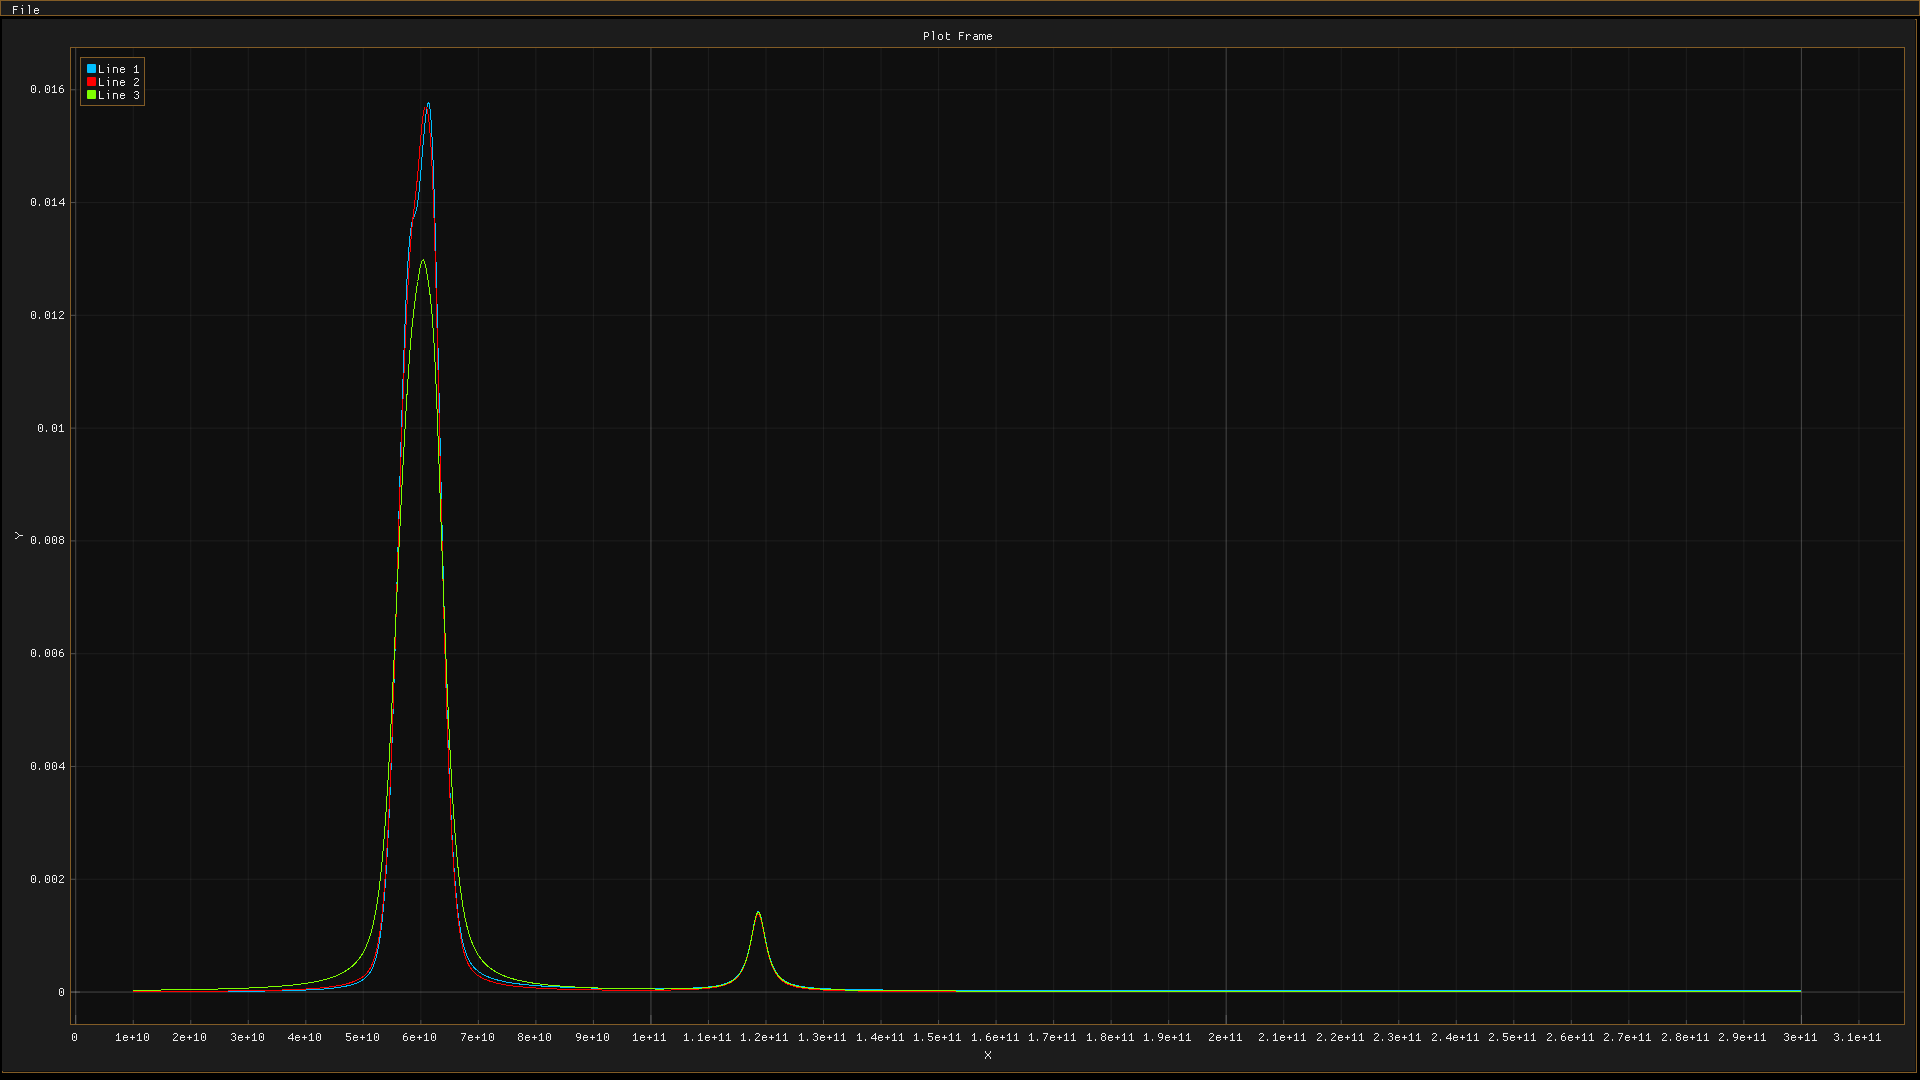
\includegraphics[width=\textwidth]{Figs/debug_gui/test_gui.png}
 \caption{Example plot.  Here we show the absorption versus frequency for some
 O$_2$ absorption models.}
 \label{fig:debug_gui_test_gui}
\end{figure}

The features of the plotting tool is limited but intuitive enough to access and
view the data.

There are three components to the plotting tool.  The plot frame is where your data
is displayed.  The plot axis shows the scales of the data.  The menu bar offers
some options to manipulate the window.  Each of these have limited operations listed below.
\begin{itemize}
 \item Menu bar
  \begin{itemize}
   \item \shortcode{File} --- access meta information about the window and data
    \begin{itemize}
     \item \shortcode{Fullscreen} (shortcut F11) takes the plotting window fullscreen.  The exit fullscreen mode, use escape, F11, quit the application or press the fullscreen menu item again.
     \item \shortcode{Export Data} (shortcut Ctrl+S) saves the Y-axis data to an XML-file.  In the templated code, the new file will be an ArrayOfVector, in the non-templated code it will be a simple Vector.
     \item \shortcode{Quit} (shortcut Ctrl+X) quits the application.
    \end{itemize}
  \end{itemize}
 \item Plot axis
  \begin{itemize}
   \item Double left-click: Resets the clicked axis to the maximum possible value.  Note that for values very small or very large, this might fail and you need to manually fix the axis.
   \item Double right-click: Opens the axis dropdown-menu with the following options:
    \begin{itemize}
     \item Min: Select the minimum value by writing the number in the text box, or lock the axis by ticking the checkbox.
     \item Max: Select the maximum value by writing the number in the text box, or lock the axis by ticking the checkbox.
     \item Invert: Check the box to switch the order of high-and-low along the respective axis.
     \item Log Scale: Check the box to show the axis in logarithmic scale.
     \item Time (X-axis only): Check the box to interpret the X axis as Unix time and display the relevant as dates.
     \item Grid Lines: Uncheck the box to remove grid lines in the plot frame for the axis.
     \item Tick Marks: Uncheck the box to remove tick marks in the plot frame for the axis.
     \item Labels: Uncheck the box to remove the labels from the axis.
    \end{itemize}
  \item Left-click and drag:  Moves the axis in the direction dragged.
  \item Vertical scroll:  Extends or contracts the axis range around the value where the scroll began.
  \end{itemize}
 \item Plot frame
  \begin{itemize}
   \item Double left-click: Scales both X-and-Y to a best-fit scenario (still with the caveat that very small and very large numbers might not work properly)
   \item Double right-click:  Opens a dropdown-menu with access to the plot axis dropdown-menues and some settings
   \item Scroll:  Extend or contract both axis around the point where the scoll began
   \item Left-click and drag:  Moves the axis around
   \item Right-click and drag:  Selects a region and zooms in when the right-click is let go.  If Shift is held, the zoom window is modified to include the entire Y-axis.  If Alt held, the zoom window is modified to include the entire X-axis.
   \item Legends:  In the upper left corner of the plot frame are the legends of the plot.  If hovered, the hovered line will be enlarged inside the plot frame.  If the colored check box is pressed, the line will be removed from the plot frame.
  \end{itemize}
\end{itemize}

The debug GUI is based on the \shortcode{Dear ImGui} GUI framework, with \shortcode{ImPlot}
drawing the plots and uses \shortcode{imgui-filebrowser} to deal with the filesystem.
